% -----------------------------------------------------------------------------
% Auteurs : Romain de Wolff, Bruno da Silva, Gilles Meier
% -----------------------------------------------------------------------------
\documentclass[10pt,a4paper,titlepage]{article}
\usepackage[utf8]{inputenc}     % encodage des characteres en utf8
\usepackage[francais]{babel} % pour la table des matières en français 

\usepackage{url} % pour les liens internet
\usepackage[colorlinks=true,linkcolor=black,bookmarks=true,bookmarksopen=true]{hyperref} % rendre les liens clickable
\usepackage{fancyhdr}	 
\usepackage{listings} 
\lstset{language=Java, breaklines, fontadjust, inputencoding=utf8, basicstyle=\small, numbers=left, numberstyle=\tiny, tabsize=2}

\usepackage[dvips]{graphicx}
\usepackage{epstopdf}


% -----------------------------------------------------------------------------
%   Info sur le labo
% -----------------------------------------------------------------------------
\newcommand{\branchetag}{ASI}
\newcommand{\branche}{Applications et Services Internet}
% \newcommand{\labonummer}{}
\newcommand{\laboname}{SSL - JSSE (Java Secure Socket Extension)}
\newcommand{\auteurOne}{Romain de Wolff}
% \newcommand{\auteurTwo}{Bruno da Silva}
\newcommand{\promo}{IL2008}
\newcommand{\titreDocument}{Rapport de laboratoire}

% -----------------------------------------------------------------------------


% -----------------------------------------------------------------------------
% Pour l'utilisation de code
% -----------------------------------------------------------------------------

\usepackage{listings} 
%\lstset{language=Java, breaklines, fontadjust, inputencoding=utf8, basicstyle=\small, numbers=left, numberstyle=\tiny, tabsize=2}

\usepackage{courier}
\usepackage{color}

% color definitions
\definecolor{dkgreen}{rgb}{0,0.6,0}
\definecolor{gray}{rgb}{0.5,0.5,0.5}
\definecolor{lightblue}{rgb}{0.92,0.92,1}

\lstset{language=Html,
  %keywords={break,case,catch,continue,else,elseif,end,for,function,
  %   global,if,otherwise,persistent,return,switch,try,while},
  keywords={script, document, function},
  basicstyle=\ttfamily\small,
  % basicstyle=\scriptsize,
  keywordstyle=\color{blue},
  commentstyle=\color{dkgreen},
  stringstyle=\color{red},
  numbers=none,
  numberstyle=\tiny\color{gray},
  stepnumber=1,
  numbersep=10pt,
  backgroundcolor=\color{lightblue},
  tabsize=2,
  linewidth=0pt,
  showspaces=false,
  showstringspaces=false,
  frame=single,
  framexleftmargin=10pt,
  framexrightmargin=10pt,
  framexbottommargin=7pt,
  framextopmargin=7pt,
  linewidth=335pt, % largeur de la ligne de code affichée
  xleftmargin=10pt, % espace avant le debut du cadre
  aboveskip=20pt
}

% -----------------------------------------------------------------------------
% En tete et pied de page

\pagestyle{fancy} % defini nos propre header & footer
\fancyhf{} % delete current header and footer 
\fancyhead[L]{\branchetag}
\fancyhead[C]{\laboname}
\fancyhead[R]{\auteurOne} 
\fancyfoot[L]{
\includegraphics[width=3cm]{img/HEIG-VD.jpg}}
\fancyfoot[R]{\bfseries\thepage}

\renewcommand{\headrulewidth}{0.5pt} 
\renewcommand{\footrulewidth}{0.1pt} 
\addtolength{\footskip}{10.0pt} % space for the rule 
\fancypagestyle{plain}{
	\fancyhead{} % get rid of headers on plain pages 
	\fancyfoot{}
	\renewcommand{\headrulewidth}{0pt} % and the line 
	\renewcommand{\footrulewidth}{0pt} % and the line 
}

\author{\auteurOne}
\title{\branchetag : \laboname}
\date{\today}

\begin{document}

% -----------------------------------------------------------------------------
% Page de titre
\pagenumbering{Roman}
\pagestyle{headings}
\begin{titlepage}
	\begin{center}

	
\includegraphics[width=6cm]{img/HEIG-VD.jpg}\\
	
		\vspace{3cm}
		\LARGE \branche %Laboratoire No %\labonummer \\
		\vspace{3cm}\\
		\Huge \laboname \\
		\vspace{3cm}

		\Large \textsc{\titreDocument} \\
		\vspace{3cm}

		\large \auteurOne \\
		% \auteurTwo \\ % pour un eventuelle deuxième auteur
		\vspace{10pt}
		\normalsize \textsc{\promo} \\
		\vspace{1cm}
		\today
	\end{center}
\end{titlepage}
% -----------------------------------------------------------------------------

% -----------------------------------------------------------------------------
% Table des matières
\tableofcontents
\newpage
\pagestyle{fancy}
\pagenumbering{arabic}

% -----------------------------------------------------------------------------
\section{Introduction}
% -----------------------------------------------------------------------------
% -----------------------------------------------------------------------------
\section{Réponses aux questions}
% -----------------------------------------------------------------------------

Lors de la connexion sur notre serveur HTTPS à l'aide du navigateur Firefox, le serveur nous affiche une alerte comme le montre la figure \ref{fig:connex}

\begin{figure}[htbp]
   \begin{center}
      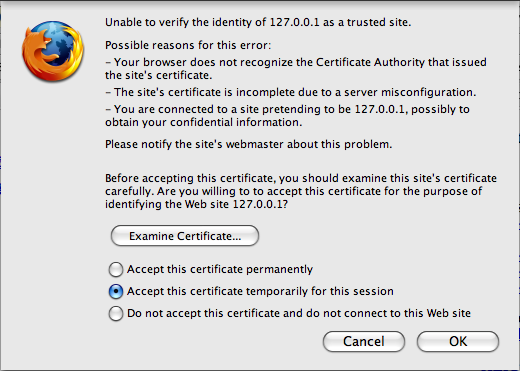
\includegraphics[width=345px]{img/1.png}
   \end{center}
   \caption{Alerte affichée lors de la connexion sur le site sécurisé.}
	\label{fig:connex}
\end{figure}

Nous acceptons ce certificat et nous allons voir le site s'afficher. On remarque que le site est sécurisé grâce à l'icone représentant un cadenas (an bas à droite dans Firefox) que l'on peut voire sur la figure \ref{fig:icone}.

\begin{figure}[htbp]
   \begin{center}
      
\includegraphics[height=23px]{img/2.png}
   \end{center}
   \caption{Icone dans la barre des tâches du navigateur Firefox.}
	\label{fig:icone}
\end{figure}

En cliquant sur le cadenas on peut afficher les informations relatives à la sécurité et donc du certificat que l'on a accepté. La figure \ref{fig:infosecu} nous montre à quoi ressemble cette fenêtre.

\begin{figure}[htbp]
   \begin{center}
      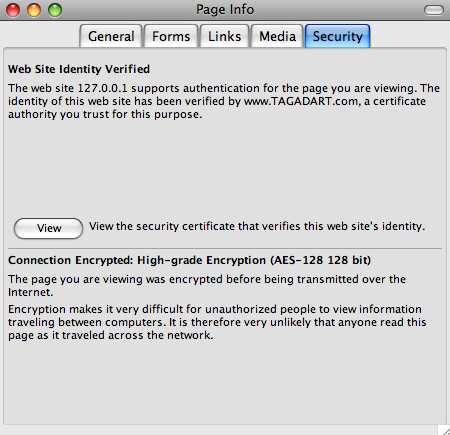
\includegraphics[width=345px]{img/3.png}
   \end{center}
   \caption{Information sur la sécurité du site.}
	\label{fig:infosecu}
\end{figure}


\begin{figure}[htbp]
   \begin{center}
      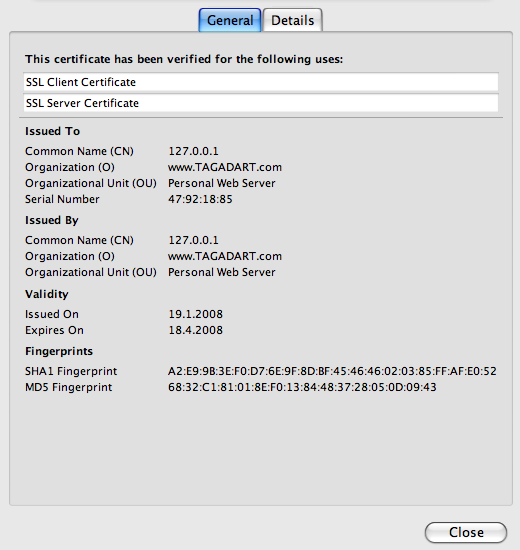
\includegraphics[width=345px]{img/4.png}
   \end{center}
   \caption{Affichage détaillée des informations sur le certificats que nous avons créé.}
	\label{fig:certif}
\end{figure}

\subsection{En examinant le certificat du serveur, comment pouvez-vous en déduire que celui-ci est auto-signé?}

\subsection{Pourquoi serait-il intéressant de faire signer le certificat par une entité comme Verisign?}

% -----------------------------------------------------------------------------
\section{Clé publique}
% -----------------------------------------------------------------------------

\scriptsize{
\begin{verbatim}
-----BEGIN NEW CERTIFICATE REQUEST-----
MIIBujCCASMCAQAwejELMAkGA1UEBhMCQ0gxCzAJBgNVBAgTAlZEMREwDwYDVQQHEwhMYXVzYW5u
ZTEZMBcGA1UEChMQd3d3LlRBR0FEQVJULmNvbTEcMBoGA1UECxMTUGVyc29uYWwgV2ViIFNlcnZl
cjESMBAGA1UEAxMJMTI3LjAuMC4xMIGfMA0GCSqGSIb3DQEBAQUAA4GNADCBiQKBgQCjcLrCVl/h
50CuSHjNevhTrRS0bCQ1oCN27c3hTLdDbLVjDNqUJqziTXpowFTUXmM/hrbKwVzM5+I4krwx/6dW
oVVhaGywxkQwN4mQ2rgFvkdm8xIpPKfyVMTLYRQLfd89qLYC8C0SUR3MqzuNRpT7lnla1RB9A6Mg
IIx53mf8UQIDAQABoAAwDQYJKoZIhvcNAQEEBQADgYEAAht/hvwHdT1Qb5ZPe6EmBbMJe6VozqQT
yzaA2q6+4Y+FzuQ0PT7oePyg22e6HTiEtxRIhNGiCXVlceeNxKYFBGoBGVSGOHvauWFGRntErntQ
X7vYKW5XCjHfEpsMwKsj42b4zMFn743IT/LmiC/NsghW3q+UD7AUslld4+XaX68=
-----END NEW CERTIFICATE REQUEST-----
\end{verbatim}
}

% -----------------------------------------------------------------------------
\section{Conclusion}
% -----------------------------------------------------------------------------



% -----------------------------------------------------------------------------
\section{Références}
% -----------------------------------------------------------------------------

\small
\begin{description}
	\item[\url{http://jquery.com/}] {Site officiel de jQuery.}
	\item[\url{http://www.jquery.info/}] {Site francophone sur jQuery.}
	\item[\url{http://docs.jquery.com/Tutorials}] {Tutoriels officiels.}
	\item[\url{http://www.gotapi.com/html}] {Description de l'API jQuery ainsi que HTML. Très utile comme référence rapide et disponibles pour une grande variété de langages courants.}
	\item[\url{http://developer.mozilla.org/fr/docs/Le_DOM_et_JavaScript}] {Explication du DOM et JavaScript.}
	\item[\url{http://www.yoyodesign.org/doc/w3c/dom2-core/introduction.html}] {Documentation DOM.}
	\item[\url{http://fr.wikipedia.org/wiki/Document_Object_Model}] {Documentation DOM.}
	\item[\url{http://fr.wikipedia.org/wiki/Javascript}] {Documentation JavaScript.}
\end{description}
\end{document}